\documentclass[OPS,lsstdraft,authoryear,toc]{lsstdoc}
% GENERATED FILE -- edit this in the Makefile
\newcommand{\lsstDocType}{RTN}
\newcommand{\lsstDocNum}{092}
\newcommand{\vcsRevision}{3df8314-dirty}
\newcommand{\vcsDate}{2025-01-15}


% Package imports go here.

% Local commands go here.
\newcommand\schedview{\texttt{schedview }}
\newcommand\todo[1]{\textcolor{red}{TODO: #1}}

%If you want glossaries
%\input{aglossary.tex}
%\makeglossaries

\title{schedview: Tools for Visualizing Survey Progress and Scheduler Performance}

% This can write metadata into the PDF.
% Update keywords and author information as necessary.
\hypersetup{
    pdftitle={schedview: Tools for Visualizing Survey Progress and Scheduler Performance},
    pdfauthor={Eric H. Neilsen, Jr.},
    pdfkeywords={}
}

% Optional subtitle
% \setDocSubtitle{A subtitle}

\author{Eric H. Neilsen, Jr.}

\setDocRef{RTN-092}
\setDocUpstreamLocation{\url{https://github.com/lsst/rtn-092}}

\date{\vcsDate}

% Optional: name of the document's curator
% \setDocCurator{The Curator of this Document}

\setDocAbstract{%
\texttt{schedview} is a python module with tools for collecting, processing, and visualizing survey progress and scheduler performance metadata for the Legacy Survey of Space and Time (LSST). These components can be combined into online dashboards (or other user interfaces), used within jupyter notebooks, or with automatically generated parameterized notebooks using tools such as Times Square. The current version includes the pre-night briefing, a report that summarizes a simulation of a night of observing before it takes place to catch problems and prepare staff for the night ahead; the scheduler snapshot dashboard, a web application for examining the state of the scheduler at different times during observing; and the scheduler-focused night summary, which summarizes a completed night. Examples of figures supported for these dashboards and reports include interactive sky maps of visits, basis function evaluations used by the scheduler, timelines of visits and logging events, plots of visit metadata, and others.
}

% Change history defined here.
% Order: oldest first.
% Fields: VERSION, DATE, DESCRIPTION, OWNER NAME.
% See LPM-51 for version number policy.
\setDocChangeRecord{%
  \addtohist{1}{YYYY-MM-DD}{Unreleased.}{Eric Neilsen}
}


\begin{document}

% Create the title page.
\maketitle
% Frequently for a technote we do not want a title page  uncomment this to remove the title page and changelog.
% use \mkshorttitle to remove the extra pages

\section{Introduction} \label{sec:intro}

Over the course of ten years of observing, the NSF-DOE Vera C. Rubin Observatory, funded by the U.S. National Science Foundation and the U.S. Department of Energy's Office of Science, will complete the Legacy Survey of Space and Time (LSST), collecting approximately 2 million images over the 18000 square degree footprint in the southern sky. Each image will be constructed from a single visit, where a visit is a set of one or more consecutive exposures on the sky with the same pointing and filter. An automated scheduler, \texttt{rubin\_scheduler}, will select which visit will be taken at any given time. A wide range of factors influence which visit should be selected for observing at any given time. These factors include physical possibility (e.g., is the pointing on the sky beneath the horizon?); conditions affecting data quality (e.g., exposures using the u, g, or r filter will be more adversely affected by bright moonlight than those in i, z, or y); efficiency (spending a lot of time slewing means fewer exposures and less data in the survey); and suitability for the wide variety of science the survey will support (e.g., uniformity in depth over the footprint and observing cadence). This complexity makes it challenging to understand and assess the scheduler's behavior at any given time.

A variety of people working on Rubin Observatory and the LSST require tools to help them monitor and explore scheduler behavior and survey progress, in a variety of contexts: both the scheduling team and observatory staff preparing for a night of observing need to assess the readiness of the scheduler and develop expectations for nominal behavior during the night; observatory staff will also need to explore the scheduler state during the night to monitor it for problems and understand its behavior, and sometime diagnose problems; and the observatory staff and the scheduling team will need to assess scheduler performance on completed night of observing. Both the scheduling team and management will need to assess and report on survey progress over longer time scales, and produce reports for a variety of audiences. Tools for examination of scheduler behavior and survey progress therefore need to support users with a variety of levels of expertise on the scheduler, from novice to expert. The tools need to be suitable for analysis on a variety of time-scales, and will need to be run using data accessible from different sites with clients run at different sites.

\schedview is a python package of tools for examining, assessing, and monitoring the scheduler and its behavior, designed to be flexible enough to meet these requirements. The architecture divides the functionality into different elements that can be mixed and matched to be suitable for different audiences, environments, and uses, such that different reports for different audiences and uses can be made using a common set of code.

\section{The Rubin Observatory scheduler} \label{sec:scheduler}

The ``feature-based scheduler'' (FBS), implemented in the \texttt{rubin\_scheduler} python package, implements the algorithm that selects visits for science operations. The \texttt{CoreScheduler} class implements the interface over which visits are queried. An instance of the \texttt{CoreScheduler} has a collection of ``surveys'' organized into ``tiers'' reflecting the priority these surveys have. Figure~\ref{fig:schedclass} shows instance diagram of an example instance of a \texttt{CoreScheduler}. The example is much simpler than realistic examples, but is complex enough to show the fundamental features of the architure.


\begin{figure}
    \centering
    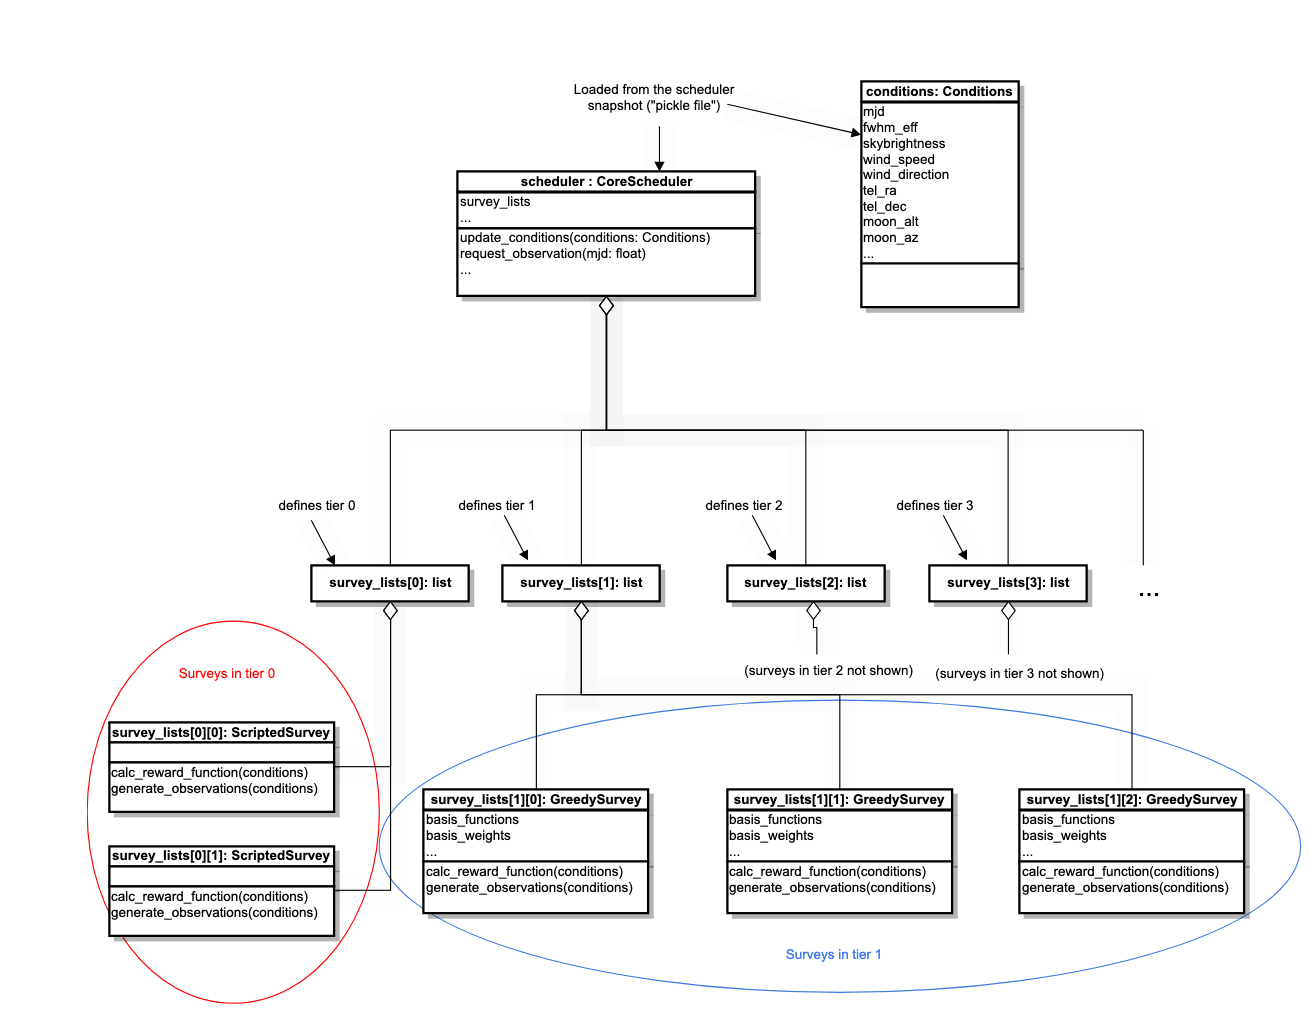
\includegraphics[width=1.0\linewidth]{schedclass.png}
    \caption{Simplified scheduler class diagram}
    \label{fig:schedclass}
\end{figure}



\begin{figure}
    \centering
    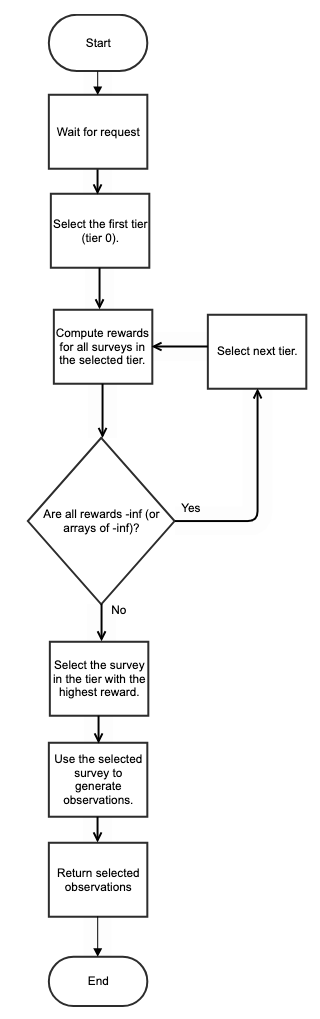
\includegraphics[width=0.35\linewidth]{schedprocess.png}
    \caption{Process for scheduler visit selection}
    \label{fig:schedprocess}
\end{figure}

Figure~\ref{fig:schedprocess} shows the process by which the scheduler selects visits.
For any set of conditions, each ``survey'' has an associated reward. A reward may either be a scalar or a map of values over the sky (as a healpix map).
When the reward (if it is a scalar) or the maximum value of the reward (if it is a map) is a number greater than \texttt{-Infinity}, that survey can also supply an observation or list of observations to be scheduled.
When the reward (or maximum value of the reward) for the survey is \texttt{-Infinity}, this means that all observations supplied by the survey are infeasible under the provided conditions.

When the \texttt{CoreScheduler} is asked to schedule an observation for a given set of conditions, it works through each tier in order until it finds a tier with at least one survey that can supply an observation. Among all of the surveys in this tier, it selects the one which returns the highest value for the reward, and returns the observation selected by that survey. Figure~\ref{fig:schedprocess} provides a visual demonstration of the steps in this process.

Most surveys compute rewards using a weighted sum of basis functions. A basis function is a function of the conditions (time, weather, etc.) computed for, and by, a survey. Basis functions can either return scalar values or maps of the sky (as healpix arrays).

\begin{figure}
    \centering
    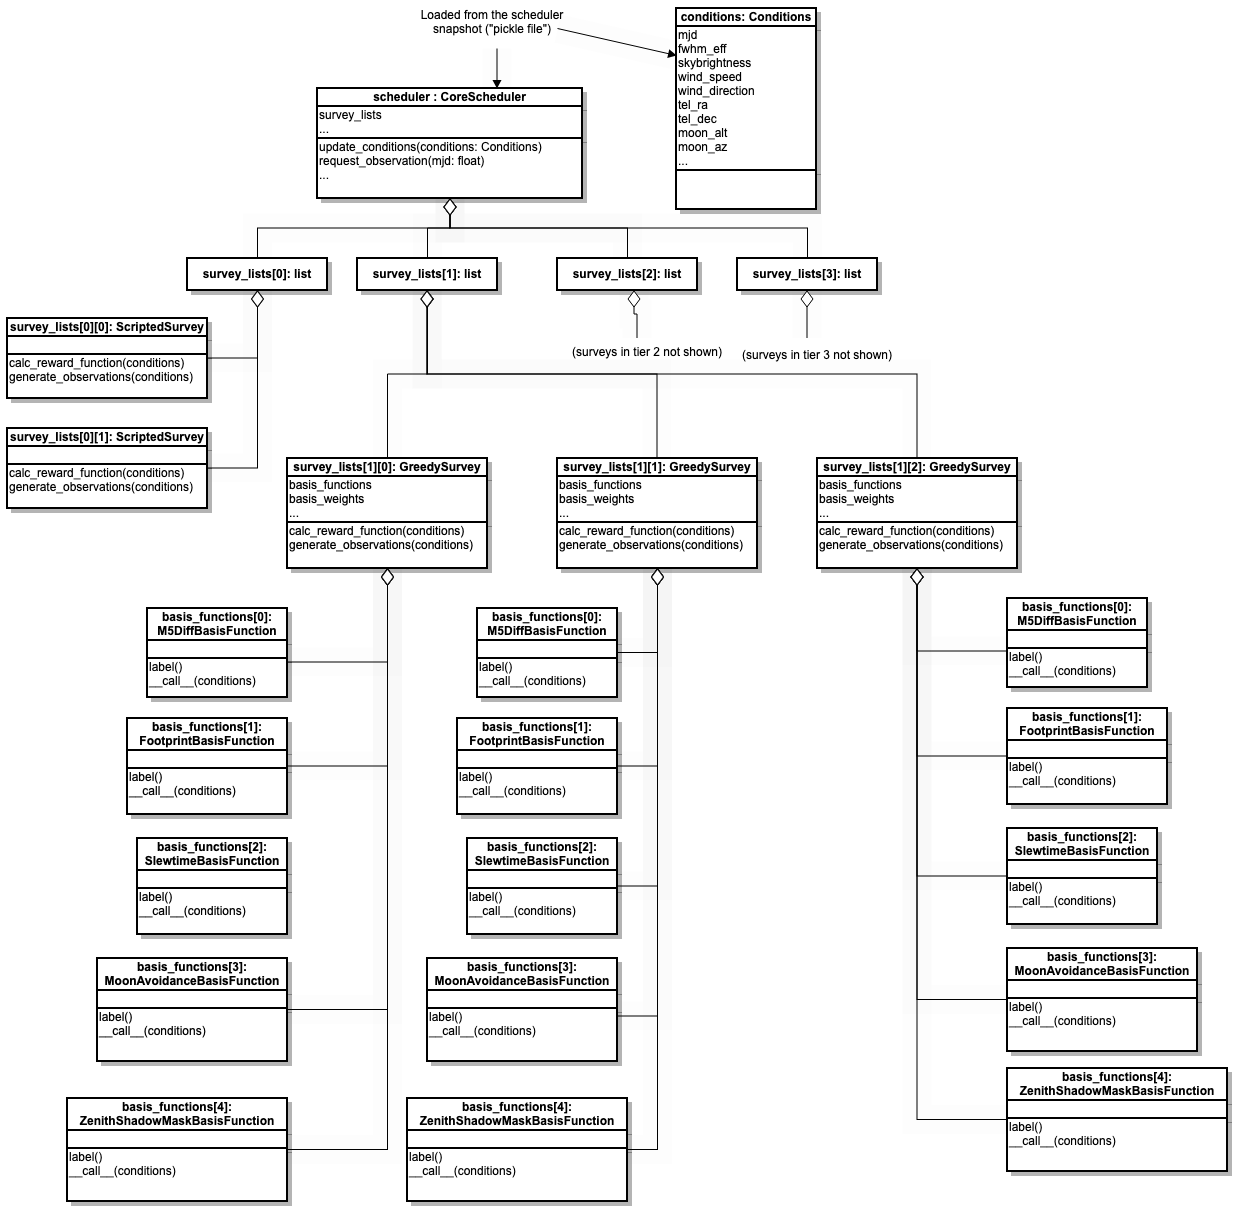
\includegraphics[width=1.0\linewidth]{schedinst.png}
    \caption{Scheduler instance diagram showing included surveys}
    \label{fig:schedinst}
\end{figure}

Figure~\ref{fig:schedinst} expands on the previous diagram, displaying the set of instances of basis functions belonging to each survey. They will often be similar from one survey to another (instances of the same classes), but they can have different configurations. For example, different surveys might select observations in different filters, in which case the instance of \texttt{M5DiffBasisFunction} for one survey will be different from the instance of \texttt{M5DiffBasisFunction} for another. In other cases, they might be exact copies.

\begin{figure}
    \centering
    \begin{tabular}{|l|l|l|l|} \hline
         \multirow{15}{*}{\texttt{CoreScheduler}} &  \multirow{2}{*}{tier 0} & [0] Scripted survey & - \\ \cline{3-4}
          &                          & [1] Scripted survey                & - \\  \cline{2-4}
          & \multirow{10}{*}{tier 1} & \multirow{5}{*}{[0] Greedy survey} & [0] M5Diff\_r \\ \cline{4-4}
          &                          &                                    & [1] Footprint\_r \\  \cline{4-4}
          &                          &                                    & [2] Slewtime\_r \\  \cline{4-4}
          &                          &                                    & [3] MoonAvoidance \\ \cline{4-4}
          &                          &                                    & [4] ZenithShadowMask \\ \cline{3-4}
          &                          & \multirow{5}{*}{[1] Greedy survey} & [0] M5Diff\_i \\  \cline{4-4}
          &                          &                                    & [1] Footprint\_i \\  \cline{4-4}
          &                          &                                    & [2] Slewtime\_i \\ \cline{4-4}
          &                          &                                    & [3] MoonAvoidance \\ \cline{4-4}
          &                          &                                    & [4] ZenithShadowMask \\ \cline{3-4}
          &                          & [2] Greedy survey                  & ... \\ \cline{2-4}
          & tier 2                   & ...                                & ... \\ \cline{2-4}
          & tier 3                   & ...                                & ... \\ \hline
    \end{tabular}
    \caption{A tabular presentation of the nested organization of the \texttt{rubin\_scheduler}'s \texttt{CoreScheduler}, tiers, surveys, and basis functions}
    \label{tab:schedinsttab}
\end{figure}

The relationships represented in Figure~\ref{fig:schedinst} can also be represented as a table, shown in Figure~\ref{tab:schedinsttab}.

In this example, the \texttt{CoreScheduler} has several tiers, each containing at least one survey, with some surveys' rewards (in this example, the instances of \texttt{GreedySurvey}) computed from several basis functions, and other surveys' rewards (the instances of \texttt{ScriptedSurvey}) computed without using basis functions.

Basis function labels are constructed from their classes and other elements of their configuration. For example, a basis function with the label \texttt{M5Diff\_r} is an instance of the \texttt{M5DiffBasisFunction} configured for the r filter. Not all configuration parameters of basis functions are necessarily represented in the label.

When all basis functions for a survey return scalars, the reward returned by the survey is also a scalar:

\begin{equation}
\textrm{reward} = \sum_{i=0}^{n} \textrm{weight}_{i} \times \textrm{basis\_function}_{i}(\textrm{conditions)}
\end{equation}

If \texttt{reward = -Infinity} for a given conditions, the survey cannot supply observations to be scheduled under those conditions. Note that this will happen any time any of the basis function values is \texttt{-Infinity}.

When at least some basis functions return healpix arrays (representing maps of the sky), the reward is also a healpix array. The value for each healpixel (identified by an id, hpid) is an independent weighted sum of corresponding healpixel values in the basis functions (and the scalar values, for any scalar basis functions):

\begin{equation}
\textrm{reward[hpid]} = \sum_{i=0}^{n} \textrm{weight}_{i} \times 
\begin{cases}
\textrm{basis\_function}_{i}(\textrm{conditions}) & \textrm{if basis\_function}_i(\textrm{conditions}) \textrm{ is a scalar} \\
\textrm{basis\_function}_{i}(\textrm{conditions})\textrm{[hpid]} & \textrm{if basis\_function}_i(\textrm{conditions}) \textrm{ is a healpix array}
\end{cases}
\end{equation}

If \texttt{reward[hpid] = -Infinity} for a given set of conditions, the survey cannot supply observations in that healpixel under those conditions. If \texttt{reward[hpid] = -Infinity} for all values of \texttt{hpid} (all healpixels = the entire sky), the survey cannot supply any observations to be scheduled under those conditions.

If, given a set of conditions, a basis function returns either a value of \texttt{-Infinity} or a healpix array that is \texttt{-Infinity} everywhere, then that basis function is said to be infeasible. Similarly, if, given a set of conditions, the reward for a survey is either \texttt{-Infinity} or is a healpix array that is \texttt{-Infinity} everywhere, then that survey is said to be infeasible.

If any of a survey's basis functions are infeasible, the survey as a whole will be infeasible. The converse, however, is not always true. It is possible for all of a survey's basis functions to be feasible, while the survey itself is not feasible. This can occur if all entries in the survey reward healpix array (i.e. the entire sky) are \texttt{-Infinity}, but different healpixels are \texttt{-Infinity} due to different basis functions, as shown in Figure~\ref{fig:bfinfeas}: while each of the individual basis functions are feasible due to non \texttt{-Infinity} healpixels, every healpixel is \texttt{-Infinity} format least one basis function, resulting in the overall survey reward being \texttt{-Infinity} everywhere.


\begin{figure}
    \centering
    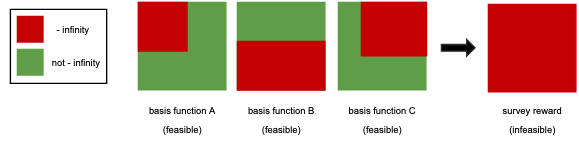
\includegraphics[width=0.5\linewidth]{bfsubsets.png}
    \caption{Demonstration of a collection of feasible basis functions that lead to an infeasible survey}
    \label{fig:bfinfeas}
\end{figure}



\appendix
% Include all the relevant bib files.
% https://lsst-texmf.lsst.io/lsstdoc.html#bibliographies
\section{References} \label{sec:bib}
\renewcommand{\refname}{} % Suppress default Bibliography section
\bibliography{local,lsst,lsst-dm,refs_ads,refs,books}

% Make sure lsst-texmf/bin/generateAcronyms.py is in your path
\section{Acronyms} \label{sec:acronyms}
\addtocounter{table}{-1}
\begin{longtable}{p{0.145\textwidth}p{0.8\textwidth}}\hline
\textbf{Acronym} & \textbf{Description}  \\\hline

DOE & Department of Energy \\\hline
LSST & Legacy Survey of Space and Time (formerly Large Synoptic Survey Telescope) \\\hline
NSF & National Science Foundation \\\hline
OPS & Operations \\\hline
RTN & Rubin Technical Note \\\hline
\end{longtable}

% If you want glossary uncomment below -- comment out the two lines above
%\printglossaries





\end{document}
